% Sample file for AES paper
\documentclass[fleqn]{jaes}

% Metadata Information
\jyear{2021}
\jmonth{June}
%\jvol{69}
%\jnum{3}

\usepackage{amsmath}\setlength{\mathindent}{10pt}
\usepackage{bm}
\usepackage{hyperref}
\usepackage{subfig}
% \usepackage{draftwatermark}
% \SetWatermarkText{DRAFT}
% \SetWatermarkColor[gray]{0.9}
% \SetWatermarkScale{1.4}
\usepackage{xcolor}
\usepackage{amssymb}

\def\SBcomment[#1]{\textcolor{red}{#1}}
\def\SWcomment[#1]{\textcolor{blue}{#1}}
\def\MDcomment[#1]{\textcolor{green}{#1}}
\def\SScomment[#1]{\textcolor{orange}{#1}}

\def\ctxt{\text{c}} %connection subscript (text)
\def\stxt{\text{s}} %string subscript (text)
\def\ptxt{\text{p}} %plate subscript (text)
\def\mtxt{\text{m}} %mass subscript (text)
\def\itxt{\text{i}} %point of 'interest' subscript (text)
\def\Btxt{\text{B}} %bow subscript (text)
\def\etxt{\text{e}} %excitation subscript (text)
\def\rtxt{\text{r}} %lip reed subscript (text)
\def\ttxt{\text{t}} %tube subscript (text)

\def\sgn{\text{sgn}}
\def\sm{\text{sm}} %string-mass interaction tromba
\def\mp{\text{mp}} %mass-plate interaction tromba

\def\MoneD{{\mathcal{M}^n}}
\def\MtwoD{{\mathcal{M}_2^n}}

\def\Nfrac{\mathcal{N}}
\def\flip{\leftarrow}
\def\Ucal{\mathbfcal{U}}

% states
\def\uln{u_l^n}
\def\wln{w_l^n}
\def\wmn{w_m^n}
\def\un{u^n}
\def\ulmn{u_{l,m}^n}
\def\ulm{u_{l,m}}
\def\uqn{u_q^n}
\def\qlmn{q_{l,m}^n}

\def\wlmn{w_{l,m}^n}
\def\zlmn{z_{l,m}^n}
\def\ubr{u_\text{br}}
\def\zbr{z_\text{br}}

\def\qln{q_l^n}
\def\lu{{l_u}}
\def\lw{{l_w}}
\def\ulun{u_\lu^n}
\def\ulcn{u_{l_\ctxt}^n}
\def\wlwn{w_\lw^n}
\def\wmcn{w_{m_\ctxt}^n}

\def\wmn{w_m^n}

\def\Psiln{\Psi_l^n}
\def\Psinp{\Psi_l^{n+1}}
\def\Psinm{\Psi_l^{n-1}}
\def\Psilp{\Psi_{l+1}^n}
\def\Psilm{\Psi_{l-1}^n}

% bold symbols (state vectors and matrices)
\def\u{\mathbf{u}}
\def\w{\mathbf{w}}
\def\q{\mathbf{q}}
\def\v{\mathbf{v}}
\def\z{\mathbf{z}}
\def\Z{\mathbf{Z}}
\def\I{\mathbf{I}}
\def\A{\mathbf{A}}
\def\B{\mathbf{B}}
\def\C{\mathbf{C}}
\def\Q{\mathbf{Q}}
\def\U{\mathbf{U}}
\def\J{\mathbf{J}}
\def\i{\mathbf{i}}
\def\j{\mathbf{j}}
\def\BB{\mathbfcal{B}^n}


% interpolators
\def\Iu{I_{l, u}(x_\ctxt)}
\def\Iw{I_{m, w}(\chi_\ctxt)}
\def\Ju{J_{l, u}(x_\ctxt)}
\def\Jw{J_{m, w}(\chi_\ctxt)}
\def\Iq{I_q(\chi_\ctxt)}
\def\Ilm{I_{l,m}(x_\ctxt)}

\def\uStack{\boldsymbol{u}}
\def\qq{\boldsymbol{q}}

% mathfraks
\def\H{\mathfrak{H}}
\def\h{\mathfrak{h}}
\def\t{\mathfrak{t}}
\def\b{\mathfrak{b}}
\def\p{\mathfrak{p}}
% continuous operators
\def\ptt{\partial_t^2} 
\def\pxx{\partial_x^2}
\def\pxxx{\partial_x^3}
\def\pxxxx{\partial_x^4}

\def\pyy{\partial_y^2}

\def\pt{\partial_t} 
\def\px{\partial_x} 
\def\py{\partial_y} 

% discrete operators
\def\dtt{\delta_{tt}} 
\def\dxx{\delta_{xx}}
\def\dxxx{\delta_{xxx}}
\def\dxxxx{\delta_{xxxx}}
\def\dcc{\delta_{\chi\chi}}
\def\dcccc{\delta_{\chi\chi\chi\chi}}

\def\dtd{\delta_{t\cdot}} 
\def\dtp{\delta_{t+}} 
\def\dtm{\delta_{t-}} 

\def\dxd{\delta_{x\cdot}} 
\def\dxp{\delta_{x+}} 
\def\dxm{\delta_{x-}} 
\def\dyd{\delta_{y\cdot}} 
\def\dyp{\delta_{y+}} 
\def\dym{\delta_{y-}} 

\def\mtt{\mu_{tt}} 
\def\mtd{\mu_{t\cdot}} 
\def\mtp{\mu_{t+}} 
\def\mtm{\mu_{t-}} 

\def\mxx{\mu_{xx}} 
\def\mxd{\mu_{x\cdot}} 
\def\mxp{\mu_{x+}} 
\def\mxm{\mu_{x-}} 

\def\dDelta{\delta_{\Delta}}
% \def\dDbox{\delta_{\Delta\boxplus}}
\def\dyy{\delta_{yy}}

% matrix operators
\def\Dxx{\mathbf{D}_{xx}}
\def\Dyy{\mathbf{D}_{yy}}
\def\DDxx{\mathbfcal{D}_{xx}^n}
\def\DDyy{\mathbfcal{D}_{yy}^n}
\def\Dxxxx{\mathbf{D}_{xxxx}}
\def\DDxxxx{\mathbfcal{D}_{xxxx}^n}
\def\DDdelta{\mathbfcal{D}_{\Delta}^n}

\def\DDeltamat{\mathbf{D}_\Delta}
\def\DDeltaDelta{\mathbf{D}_{\Delta\Delta}}
\def\DDDelta{\mathbfcal{D}_{\Delta}^n}
\def\DDDeltaDelta{\mathbfcal{D}_{\Delta\Delta}^n}


% often-used variables
\def\sz{\sigma_{0}}
\def\so{\sigma_{1}}
\def\vrel{v_\text{rel}}
\def\Sbar{\bar{S}}
\def\Sm{S_{l-1/2}}
\def\Sp{S_{l+1/2}}

\def\szX[#1]{\sigma_{0,{#1}}}
\def\soX[#1]{\sigma_{1,{#1}}}

\def\fs{f_\text{s}}
\def\el{\epsilon_\text{l}}
\def\er{\epsilon_\text{r}}
% mathcals
\def\D{\mathcal{D}}
\def\L{\mathcal{L}}
\def\OO{\mathcal{O}}
\def\S{\mathcal{S}}

% flooring ceiling
\def\floor[#1]{\left\lfloor #1 \right\rfloor}
\def\ceil[#1]{\left\lceil #1 \right\rceil}
\def\ansatz{\ \overset{\mathcal{A}}{\Longrightarrow}\ }
% other
\def\qaq{\quad \text{and} \quad}
\def\qwiq{\quad \text{with} \quad}
\def\qwhq{\quad \text{where} \quad}

\def\mystrut{\rule[-.2\baselineskip]{0pt}{\baselineskip}}

\def\th{\textsuperscript{th} }
\def\thOrder{\textsuperscript{th}-order }

\def\boldPhi{\boldsymbol{\phi}}
\def\boldPsi{\boldsymbol{\Psi}}
\def\eig{\text{eig}}

\def\Dxx{\mathbf{D}_{xx}}
\def\alf{'}
\def\DxxA{\Dxx\alf}
\def\DyyA{\Dyy\alf}
\def\DxxxxA{\Dxxxx\alf}
\def\DDeltamatA{\DDeltamat\alf}
\def\DDeltaDeltaA{\DDeltaDelta\alf}
\def\Aterm{\mathcal{A}^n}
\DeclareMathAlphabet{\mathcal}{OMS}{ntxsy}{m}{n}   % or txsy
\DeclareMathAlphabet\mathbfcal{OMS}{cmsy}{b}{n} % for paper A

\makeatletter
\renewcommand*\env@matrix[1][*\c@MaxMatrixCols c]{%
  \hskip -\arraycolsep
  \let\@ifnextchar\new@ifnextchar
  \array{#1}}
\makeatother

\begin{document}

% Page heads
\markboth{WILLEMSEN ET AL.}{THE DYNAMIC GRID}

% Title portion
\title{The Dynamic Grid: Time-Varying Parameters for Musical Instrument Simulations based on Finite-Difference Schemes}
% \title{Physical Morphing: Dynamic Grids for Finite-Difference Schemes}
% \title{A Framework for Dynamic Grids for Finite-Difference Schemes in Musical Instrument Simulations}
%Author Info.
\authorgroup{
\author{SILVIN WILLEMSEN,\textsuperscript{1}} \author{STEFAN BILBAO,\textsuperscript{2}} \author{MICHELE DUCCESCHI,\textsuperscript{3}} AND \author{STEFANIA SERAFIN\textsuperscript{1}}
\email{(sil@create.aau.dk)\quad\quad\quad\quad (s.bilbao@ed.ac.uk)\ \  \quad\quad(michele.ducceschi@unibo.it)\quad\quad\quad\quad\quad\quad\quad (sts@create.aau.dk) }
\affil{\textsuperscript{1}Multisensory Experience Lab, CREATE, Aalborg University Copenhagen, Denmark \\
\textsuperscript{2}Acoustics and Audio Group, University of Edinburgh, Scotland\\
\textsuperscript{3}Department of Industrial Engineering (DIN), University of Bologna, Italy}
}

%Abstract
\abstract{% 
Physical modelling of musical instruments is a well-established field and many modelling techniques exist. Finite-difference time-domain (FDTD) methods are known for their generality and flexibility in terms of the systems one can model, but are inflexible to smooth parameter variations due to their reliance on a static grid. 
% The field of physically modelling musical instruments, though well-established, contains relatively little work on physically impossible manipulations of the virtual instrument. One could potentially change material properties and geometry of the underlying instrument
This paper presents the dynamic grid, a method to smoothly change grid configurations of FD schemes based on (sub-audio rate) time-varying parameters. This allows for physically impossible manipulations of material properties and geometry of the now-virtual instrument, and could potentially broaden the range of expression for the musician. The method is applied to the 1D wave equation and the stiff string, as well as to 2D systems, including the 2D wave equation and the thin plate. Results show that the method does not introduce `visible' artifacts when changing between grid configurations.
Future work includes stability analysis and real-time implementation and control.
}
\maketitle
%Head 1
\section{INTRODUCTION}\label{sec:introduction}

Nearly all musical instruments can be subdivided in an exciter and a resonator component \cite{Borin1989}. Examples of resonators are the violin and the trumpet, which are excited by the bow and the lips of the player respectively. The resonator is usually assumed to be linear and time-invariant, whereas the excitation usually contains a nonlinear component and can be controlled by the performer over time. Over the past few decades, much work has been done on virtualising real-world musical instruments, specifically resonator components, through various physical modelling techniques. Many techniques exist, of which finite-difference time-domain (FDTD) methods are considered the most flexible and generalisable in terms of the systems one can model \cite{Bilbao2009}.

Although FDTD methods have been extensively used for sound synthesis purposes, relatively little work has been done on varying the defining parameters of the resonator during performance. First of all, this is due to the difficulties that arise when working with time-varying systems, both in the underlying continuous equations, as well as stability issues arising in their numerical implementation. Secondly, most physical systems at hand are described by a fixed set of parameters. In other words, properties such as material density and geometry of the instrument are unchangeable in the real world, and will thus remain this way in simulation.

There do exist real-world cases where the defining parameters of the resonator are time-varying.
A notable example is the trombone, where the length of the acoustic tube is changed during performance. Furthermore, membrane tension in timpani or ``hourglass drums"\footnote{Ayan Bisi Adeleke - Master talking drummer - drum talks: \url{https://youtu.be/B4oQJZ2TEVI?t=9}} are varied and thus face the same difficulties when modelled using FDTD methods. See \cite[Sec. 12.4]{Willemsen2021Thesis} for more examples. An acoustic tube with time-varying length implemented using FDTD methods is presented in \cite{Hofmann2019} and uses full-grid interpolation to update the system states whenever the length is changed. Grid points are added and removed at the radiating end.

To the authors' opinion, one of the greatest potentials of modelling musical instruments is to exploit the virtual nature of the instrument and go beyond what is physically possible. Instrument properties which are usually fixed could be made time-varying to create sounds impossible in the real world and potentially extend the range of expression for the musician. Already existing work on time-varying parameters in physical models using modal synthesis \cite{morrison1993mosaic} are shown in \cite{Mehes2016, Willemsen2017} and digital waveguides \cite{Smith1992} are shown in \cite{Michon2014}.

% Apart from ``unphysical" manipulations of musical instruments, 

This paper presents the dynamic grid, a method to allow for time-varying parameters in real-time simulations of musical instruments based on FDTD methods. The current work generalises the method presented in \cite{Willemsen2021a} where it is applied to the 1D wave equation, and extends it to more complex systems, such as the stiff string, and 2D systems, including the 2D wave equation and the thin plate. The method appears in part in \cite[Ch. 12]{Willemsen2021Thesis} and has been used to model the trombone, including time-varying length in \cite{Willemsen2021b}. 

At its current stage, physical accuracy and stability conditions are not the main focus of the method. Instead, efficiency and applicability to already existing models are more important for this contribution. Changes in parameter values are therefore assumed to be sub-audio rate (control rate) such that they can be applied to commonly used FD schemes.

This paper is structured as follows: Sec. \ref{sec:continuous} presents the 1D wave equation as a starting point and Sec. \ref{sec:numericalMethods} introduces FDTD methods and discusses stability and simulation quality. Sec. \ref{sec:dynamicGrid} introduces the dynamic grid and its application to the 1D wave equation and the stiff string, and Sec. \ref{sec:2D} extends the method to 2D systems. Sec. \ref{sec:analysis} presents the analysis of the method and its results after which Sec. \ref{sec:discussion} discusses and Sec. \ref{sec:conclusion} concludes.

\section{CONTINUOUS SYSTEMS}\label{sec:continuous}
A useful starting point for illustrating the dynamic grid is the 1D wave equation. Consider a system of length $L$ (in m) described by state variable $q(x, t)$ defined over space $x \in [0, L]$ and time $t \geq 0$. Its dynamics are defined by the following partial differential equation (PDE)
\begin{equation}\label{eq:1DwaveCont}
    \ptt q = c^2 \pxx q,
\end{equation}
with wave speed $c$ (in m/s). Derivatives with respect to $t$ and $x$ are denoted by $\pt$ and $\px$ respectively. In the above, $q$ can be interpreted as the transverse displacement of an ideal string, or the acoustic pressure in a cylindrical tube. The two possible choices for boundary conditions of the 1D wave equation are follows:
\begin{subequations}\label{eq:contBoundaryConditions}
\begin{alignat}{2}
    q(0, t) &= q(L, t) = 0 &&\text{(Dirichlet)},\label{eq:contDirichlet}\\
    \px q(0, t) &= \px q(L,t) = 0 \ \ &&\text{(Neumann)},\label{eq:contNeumann}
\end{alignat}
\end{subequations}
and can be interpreted as `fixed' and `free' boundaries respectively for the ideal string, or `open' and `closed' boundaries respectively for the acoustic tube.

\section{NUMERICAL METHODS}\label{sec:numericalMethods}
To discretise Eq. \eqref{eq:1DwaveCont} using FDTD methods, a spatio-temporal grid needs to be defined first. 
Time $t\geq 0$ can be discretised as $t = nk$ with temporal index $n = 0, 1, 2, \hdots$ and time-step $k = 1/f_\text{s}$ (in s) with sample rate $f_\text{s}$ (in s$^{-1}$). Space $x = [0, L]$ is subdivided into $N$ equal intervals of length $h$ (in m) -- also called the grid spacing -- according to $x = lh$ with spatial index $l\in \{0, \hdots, N\}$. 

Using these definitions, the continuous state can be approximated as $q(x,t) \approxeq \qln$ where $\qln$ is a grid function that describes the state of the system over $N+1$ grid points. Furthermore, continuous-time derivatives that appear in Eq. \eqref{eq:1DwaveCont} are approximated as
\begin{subequations}
\begin{align}
    \ptt q &\approxeq \dtt \qln \triangleq \frac{1}{k^2}\left(q_l^{n+1} - 2 \qln + q_l^{n-1}\right),\\
    \pxx q &\approxeq \dxx \qln \triangleq \frac{1}{h^2}\left(q_{l+1}^n - 2 \qln + q_{l-1}^n\right).
\end{align}
\end{subequations}

Eq. \eqref{eq:1DwaveCont} can then be discretised to the following finite-difference (FD) scheme:
\begin{equation}\label{eq:1dWaveDisc}
    \dtt \qln = c^2 \dxx \qln,
\end{equation}
which can be expanded to the following update equation
\begin{equation}\label{eq:1DwaveUpdate}
    q_l^{n+1} = 2 \qln - q_l^{n-1} + \lambda^2 \left(q_{l+1}^n -2\qln + q_{l-1}^n\right),
\end{equation}
which can be implemented in software. Here, 
\begin{equation}\label{eq:courant}
    \lambda = \frac{c k}{h}
\end{equation} is referred to as the Courant number, and is related to stability and simulation quality as will be described in Sec. \ref{sec:quality}

From Eq. \eqref{eq:1DwaveUpdate} one can observe that at the end points of the system ($l=0$, and $l=N$) grid points outside the defined domain are needed, i.e., $q_{-1}^n$ and $q_{N+1}^n$. These are referred to as \textit{virtual grid points} and can be defined by discretising the boundary conditions in Eq. \eqref{eq:contBoundaryConditions} as follows:
\begin{subequations}\label{eq:discBoundaryConditions}
\begin{alignat}{2}
    q_0^n &= q_N^n = 0 &&\text{(Dirichlet)},\label{eq:discDirichlet}\\
    \dxd q_0^n &= \dxd q_N^n = 0 \ \ &&\text{(Neumann)}.\label{eq:discNeumann}
\end{alignat}
\end{subequations}
If Dirichlet boundary conditions are used, the range of calculation simply becomes $l=\{1, \hdots, N-1\}$. In this work, only Dirichlet boundaries will be considered. 

\subsection{Matrix Form}\label{sec:matrixFormOrig}
Both for compact implementation (in MATLAB) as well as for applying the dynamic grid to more complex systems, it is useful to write the update equation in Eq. \eqref{eq:1DwaveUpdate} in matrix form.

Using Dirichlet boundary conditions, the system state at time $n$ can be written as the following $(N-1) \times 1$ column vector $\q^n = [q_1^n, \hdots, q_{N-1}^n]^T$ where $T$ denotes the transpose operation. Notice that the boundaries ($q_0^n$ and $q_N^n$) are not included in the state vector as they are 0 at all times.

Expanding $\dtt$, Eq. \eqref{eq:1dWaveDisc} can then be written in matrix form as
\begin{equation}
    \q^{n+1} = (2 \I_{N-1} + c^2 k^2 \Dxx)\q^n - \q^{n-1}
\end{equation}
with $(N-1)\times(N-1)$ matrix
\begin{equation}\label{eq:dxxMat}
    \Dxx = \frac{1}{h^2}
    \begin{bmatrix}
        \ddots & \ddots & & &\mathbf{0}\\
        \ddots & -2 & 1 & & \\
        & 1 & -2 & 1 & \\
        & & 1 & -2 & \ddots \\
        \mathbf{0}& & & \ddots & \ddots 
    \end{bmatrix},
\end{equation}
and same-sized identity matrix $\I_{N-1}$. 


\subsection{Stability and Simulation Quality}\label{sec:quality}
In order to ensure stability for the scheme in Eq. \eqref{eq:1dWaveDisc} the Courant number in Eq. \eqref{eq:courant} needs to satisfy the CFL condition:
\begin{equation}\label{eq:CFL}
    \lambda \leq 1.
\end{equation}
%
If $\lambda = 1$, Eq. \eqref{eq:1dWaveDisc} provides an exact solution to Eq. \eqref{eq:1DwaveCont}. In the case that $\lambda < 1$, numerical error is introduced, which shows in a decrease in bandwidth of the simulation and dispersive effects. 

Usually, Eq. \eqref{eq:CFL} is rewritten in terms of the grid spacing such that
\begin{equation}\label{eq:stabilityCond}
    h \geq c k,
\end{equation}
which is implemented as
\begin{equation}\label{eq:orderOfCalc}
    h:=ck, \quad N = \floor[\frac{L}{h}],\quad h = \frac{L}{N},\qaq \lambda = \frac{ck}{h}.
\end{equation}
Here, $\floor[\cdot]$ denotes the flooring operation which is necessary to ensure an integer number of intervals. Equation \eqref{eq:orderOfCalc} shows that $h$ needs to be recalculated based on integer $N$ after which $\lambda$ is calculated from this. If $L/h$ is not an integer, this means that $\lambda < 1$ yielding numerical dispersion. 

\section{THE DYNAMIC GRID}\label{sec:dynamicGrid}
As stated in Sec. \ref{sec:introduction}, the goal of this work is to introduce time-varying parameters into FDTD-based simulations. 
One can observe from the 1D wave equation that the wave speed $c$ and system length $L$ are the only parameters that can be made time-varying; the other variables, such as $h$, $\lambda$ and $N$ are derived from these physical parameters. This fact gives rise to several issues in the framework described above. 

First of all, a change in the wave speed $c$ will cause a change in $\lambda$, which causes issues regarding stability and simulation quality as detailed in Sec. \ref{sec:quality}. Secondly, and more importantly, changing $c$ (or $L$) changes the number of intervals $N$ according to Eq. \eqref{eq:orderOfCalc} and thus the number of grid points describing the state of the system. Apart from \textit{how} and \textit{where} to add or remove grid points based on the now-dynamic wave speed, this needs to happen smoothly in order to prevent audible artifacts. %Note that for the 1D wave equation it does not matter for the system behaviour whether $c$ or $L$ is changed as these are inversely proportional in terms of the fundamental frequency exhibited by the system \cite{Willemsen2021a}.\footnote{In the trombone simulation in \cite{Willemsen2021b}, there is a difference between a change in $c$ and $L$ due to the spatially varying geometry.}

In this work, a \textit{fractional} number of intervals $\Nfrac = L / h$ is proposed such that $N = \floor[\Nfrac]$. This removes the necessity of the flooring operation in Eq. \eqref{eq:orderOfCalc} (and therefore the recalculation of $h$), and allows $\lambda = 1$ at all times. Furthermore, $\Nfrac$ will potentially allow for smooth transitions between grid configurations. 

\subsection{Proposed Method}
In the following, the location of a grid point (in m from the left boundary) $q_l$ at time index $n$ will be written as $x_{q_l}^n$. Moreover, the following time-varying parameters get a superscript $n$: $L^n$, $c^n$, $h^n$, $\Nfrac^n$ and $N^n$.% and $f_0^n

As a starting point, the original system $\qln$, with $l=\{0, \hdots, N^n\}$ is split into two subsystems: $\ulun$ with $l_u=\{0, \hdots, M^n\}$ and $\wlwn$ with  $l_w=\{0, \hdots, M_w^n\}$:
\begin{subequations}\label{eq:splitFDS}
    \begin{align}
        \dtt \ulun &= (c^n)^2\dxx \ulun,\\
        \dtt \wlwn &= (c^n)^2\dxx \wlwn,
    \end{align}
\end{subequations}
which have $M^n+1$ grid points and $M_w^n+1$ grid points respectively.\footnote{It is important to note that the superscripts $n$ in $M^n$ and $M_w^n$ are unaffected by the $\dtt$ operator after expansion.} Here, $0<M^n<N^n$ and $M_w^n = N^n - M^n$ and will thus contain one more grid point than the original system. Both systems are placed on the same domain $x$ with their locations defined as
\begin{equation}\label{eq:gridLocations}
    x_{u_\lu}^n =\lu h^n, \quad x_{w_\lw}^n = L^n-(M_w^n-\lw)h^n.
\end{equation}
See Figure \ref{fig:twoFreeStrings}.
\def\figwidth{0.99}
\begin{figure}[t]
    \centering
    \subfloat[]{\label{fig:twoFreeStrings}{ 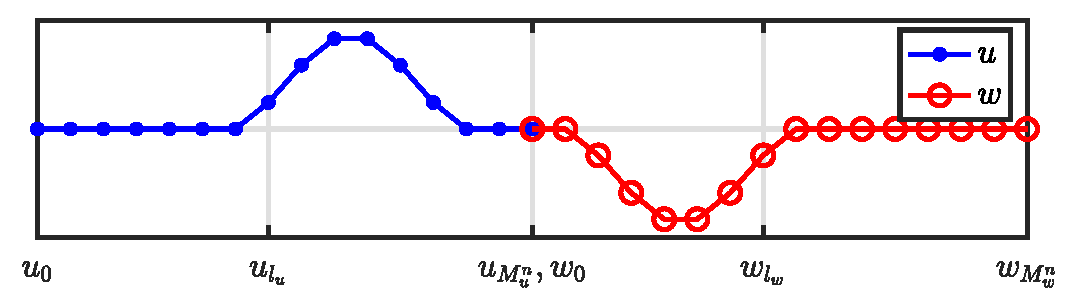
\includegraphics[width=\figwidth\columnwidth]{twoFreeStringsNarrow.eps}}}\\
    \vspace{-1em}\subfloat[]{\label{fig:twoFreeStringsGridMove}{ 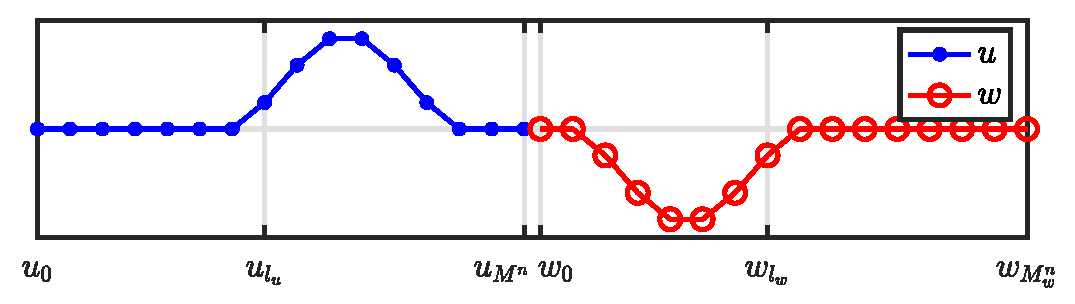
\includegraphics[width=\figwidth\columnwidth]{twoFreeStringsGridMoveNarrow.eps}}}\\
    \vspace{-1em}\subfloat[]{\label{fig:twoFreeStringsGridZoomed}{ 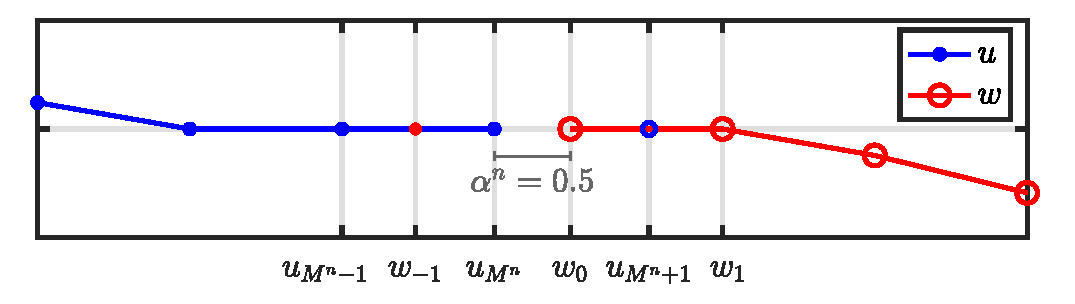
\includegraphics[width=\figwidth\columnwidth]{twoFreeStringGridMoveZoomedNarrow.eps}}}
    \vspace{-1em}\caption{Illustration of the dynamic grid. The x-axis shows the location of the respective grid points with `$x^n$' omitted for brevity. 
    (a) $\Nfrac^n = 30$. As $\Nfrac^n = N^n$, the inner boundaries overlap. (b) $\Nfrac^n = 30.5$. The wave speed $c^n$ and thus $h^n$ are decreased, $\Nfrac^n \neq N^n$ and the inner boundaries no longer overlap. (c) Figure \ref{fig:twoFreeStringsGridMove} zoomed-in. All grid points (including virtual grid points) used in Eq. \eqref{eq:connectionInterpol} are shown. The distance between the inner boundaries is expressed using $\alpha^n$ in Eq. \eqref{eq:alphaDef}.}
\end{figure}
The grid locations $\lu = 0$ and $\lw = 0$ are referred to as the \textit{outer boundaries} and, as can be observed from Eq. \eqref{eq:gridLocations}, are fixed to be at the limits of the system domain, i.e., $x_{u_0}^n = 0$ and $x_{w_{M_w^n}}^n = L^n, \forall n$. Furthermore, Dirichlet boundary conditions are imposed on the outer boundaries according to Eq. \eqref{eq:discDirichlet}. 
The grid locations $\lu = M^n$ and $\lw = 0$ are referred to as the \textit{inner boundaries}. If $\Nfrac^n = N^n$, i.e. $\Nfrac^n$ is an integer, the inner boundaries overlap and need to abide the following condition
\begin{equation}\label{eq:rigid}
    u_{M^n}^n = w_0^n, \quad \text{if}\  x_{u_{M^n}}^n =  x_{w_0}^n,
\end{equation}
which acts as a rigid connection between the inner boundaries. As shown in
\cite{Willemsen2021a}, combining this condition with Neumann boundary conditions imposed on the inner boundaries (as in Eq. \eqref{eq:discNeumann}) shows that the virtual grid points needed to calculate the $u_{M^n}^n$ and $w_0^n$ can be set according to:
\begin{equation}\label{eq:perfectOverlap}
    u_{M^n+1}^n = w_1^n, \qaq w_{-1}^n = u_{M^n-1}^n.
\end{equation}
This can be shown to yield identical behaviour to the original system.

Consider a decrease in wave speed $c^n$, which yields a decrease in $h^n$. This causes all grid points to move towards their respective outer boundary according to Eq. \eqref{eq:gridLocations} (see Figure \ref{fig:twoFreeStringsGridMove}). As the inner boundaries no longer overlap, i.e., $\Nfrac^n \neq N^n$, Eq. \ref{eq:perfectOverlap} can not be used and alternative definitions for the virtual grid points need to be found. To this end, quadratic Lagrange interpolation can be used to yield:
\begin{subequations}\label{eq:connectionInterpol}
    \begin{align}
            &u_{M^n+1}^n = \Aterm u_{M^n}^n + w_0^n - \Aterm w_1^n,
        \label{eq:calcUMP1}\\
            &w_{-1}^n = -\Aterm u_{M^n-1}^n + u_{M^n}^n+\Aterm w_{0}^n.\label{eq:calcWM1}
    \end{align}
\end{subequations}
where
\begin{equation}
    \Aterm = \frac{\alpha^n-1}{\alpha^n+1},
\end{equation}
and 
\begin{equation}\label{eq:alphaDef}
    \alpha^n = \Nfrac^n - N^n,
\end{equation}
is the fractional part of $\Nfrac^n$. Also see Figure \ref{fig:twoFreeStringsGridZoomed}.

\subsection{Matrix Form}\label{sec:matrixForm}
Similar to Sec. \ref{sec:matrixFormOrig}, system \eqref{eq:splitFDS} can be written in matrix form. The state of the subsystems can be written in vector form according to $\u = [u_1^n, u_2^n, \hdots, u_{M^n}^n]^T$ and $\w = [w_0^n, w_1^n, \hdots, w_{M_w^n-1}^n]^T$ which are $M^n \times 1$ and $M_w^n \times 1$ respectively. The full state can then be written as $\MoneD \times 1$ vector
\begin{equation}\label{eq:uStack}
    \uStack^n = \begin{bmatrix}
    \u^n\\
    \w^n
    \end{bmatrix},
\end{equation}
where $\MoneD = M^n + M_w^n$.
The update equation of the 1D wave equation including the dynamic grid can then be written in matrix form as
\begin{equation}\label{eq:1DwaveDynMatrix}
    \uStack^{n+1} = (2\I_\MoneD + (c^n)^2k^2\DDxx)\uStack^n - \uStack^{n-1} 
\end{equation}
where $\DDxx$ is an adapted version of $\Dxx$ in Eq. \eqref{eq:dxxMat} to include the quadratic interpolation presented in Eq. \eqref{eq:connectionInterpol}:
\begin{equation}\label{eq:magicMatrix}
    \!\!\!\!\!\!\DDxx = \frac{1}{(h^n)^2}\begin{bmatrix}[cccc|cccc]
     & \ddots  &\ddots & & & & \boldsymbol{0} & \\
       & \ddots & -2 & 1 & & & & \\
      & & 1 & \Aterm -2 & 1 & -\Aterm & \\ \cline{2-7}
      & & -\Aterm & 1 & \Aterm -2 & 1 & & \\
         & & & &1 & -2 & \ddots  \\
         & \boldsymbol{0} & &  &  &\ddots & \ddots &
    \end{bmatrix}
\end{equation}
and is $\MoneD \times \MoneD$. \SWcomment[something about the sizes of the quadrants and that they correspond to $M^n$ and $M_w^n$?] In the extreme case that one of the systems only has one moving grid point, e.g., if $\w^n =[w_0^n]$, the lower-right quadrant in Eq. \eqref{eq:magicMatrix} will only have one entry (being $\Aterm-2$), and the lower-left and top-right quadrants will only have one row and one column respectively. 

\subsection{Adding and Removing Points}\label{sec:addRemove}
If $c^n$ is decreased such that $N^n > N^{n-1}$, a grid point is added to the system. One can add points to either $\u$ or $\w$, or in an alternating fashion as in \cite{Willemsen2021a}, but here, only changes in $\u$ are considered. A grid point can be added to $\u$ according to
\begin{equation}
\begin{aligned}
    \u^n &= [(\u^n)^T, I_3^n\z^n]^T,\\
    \u^{n-1} &= [(\u^{n-1})^T, I_3^n\z^{n-1}]^T,\\
\end{aligned} \quad \text{if } N^n > N^{n-1}
\end{equation}
where
\begin{equation*}
    \begin{aligned}
        \z^n &= [u_{M^{n-1}-1}^n, u_{M^{n-1}}^n, w_0^n, w_1^n]^T, \quad \text{and}\\
        \z^{n-1} &= [u_{M^{n-1}-1}^{n-1}, u_{M^{n-1}}^{n-1}, w_0^{n-1}, w_1^{n-1}]^T.
    \end{aligned}
\end{equation*}
Notice that $I_3^n$ is used for adding a grid point to both $\u^n$ and $\u^{n-1}$ and that $M^{n-1}$ is used as an index for both $u^n_\lu$ and $u^{n-1}_\lu$.
Furthermore, cubic Lagrangian interpolator
\begin{equation}\label{eq:customIp}
    I_3^n = \begin{bmatrix} -\frac{\alpha^n(\alpha^n+1)}{(\alpha^n+2)(\alpha^n+3)} &\frac{2\alpha^n}{\alpha^n+2} &\frac{2}{\alpha^n+2} 
    &-\frac{2\alpha^n}{(\alpha^n+3)(\alpha^n+2)}
    \end{bmatrix},
\end{equation}
where $\alpha^n$ is as defined in Eq. \eqref{eq:alphaDef}. Notice that, as $\alpha^n \gtrsim 0$ the moment a grid point is added, $I_3^n\approx [0, 0, 1, 0]$ and the state of the added grid point is almost fully determined by the state of the inner boundary $w_0^n$. 

Removing grid points happens through simple deletion. If $c^n$ is increased such that $N^n < N^{n-1}$, a point is removed from $\u$ according to
\begin{equation}
\begin{aligned}
    \u^n &= [u_1^n, \hdots, u_{M^{n-1}-1}^n]^T,\\
    \u^{n-1} &= [u_1^{n-1}, \hdots, u_{M^{n-1}-1}^{n-1}]^T,
    \end{aligned} \quad \text{if } N^n < N^{n-1}.
\end{equation}
The limit on changing grid configurations is the addition / removal of one grid point per sample. Practically, this limit needs to be much lower to keep the system well-behaved. In \cite{Willemsen2021b}, a lower limit of 20 samples per change is used together with $\lambda = 0.999$, no artifacts 

\subsection{State Correction}\label{sec:stateCorrection}
At the moment that a point is removed, and thus $x_{u_{M^n}}^n \approxeq x_{w_0}^n$, the states of the inner boundaries might not be approximately equal, i.e., $u_M^n \not\approxeq w_0^n$. This violates the rigid connection in Eq. \eqref{eq:rigid} and -- in practice -- causes audible artifacts. To reduce this, a method of \textit{state correction}\footnote{\textit{displacement correction} in \cite{Willemsen2021a}.} is introduced and adds an artificial spring force between the inner boundaries:
\begin{align*}
    \dtt u_\lu^n = (c^n)^2\dxx u_\lu^n+ J_u(x_{u_{M^n}}^n)
    F_\text{c}^n,\\
    \dtt w_\lw^n = (c^n)^2\dxx w_\lw^n - J_w(x_{w_0}^n)
    F_\text{c}^n,
\end{align*}
where
\begin{equation}\label{eq:spreadingOperators}
    \begin{aligned}
    J_u(x_i^n)& =
    \begin{cases}
        \frac{1}{h^n}, & \lu = \lfloor x_i^n/h^n\rfloor\\
        0,& \text{otherwise}
    \end{cases}
    \quad\text{and}\\
    J_w(x_i^n) &=
    \begin{cases}
        \frac{1}{h^n}, & \lw = \lfloor x_i^n/h^n \rfloor - M^n\\
        0,& \text{otherwise}
    \end{cases}
\end{aligned}
\end{equation}
apply the correction force to the inner boundaries. 
Defining centred averaging and difference operators as
\begin{subequations}\label{eq:centredOperators}
\begin{align}\label{eq:centredAverage}
    \mu_{t\cdot}q_l^n &= \frac{1}{2} \left(q_l^{n+1} + q_l^{n-1}\right),\\
    \delta_{t\cdot}q_l^n &= \frac{1}{2k} \left(q_l^{n+1} - q_l^{n-1}\right),
\end{align}
\end{subequations}
the effect of the artificial spring can be defined as
\begin{equation}\label{eq:dispCorrForce}
    F_\text{c}^n = \beta^n \left(\mu_{t\cdot}\eta^n +\sigma_\text{sc}\delta_{t\cdot}\eta^n \right),
\end{equation}
with damping coefficient $\sigma_\text{sc}$ and
\begin{equation}\label{eq:betaDef}
    \beta^n = \beta(\alpha^n) = \frac{1-\alpha^n}{\alpha^n}.
\end{equation}
Note that Eq. \eqref{eq:betaDef} is still defined for $\alpha^n = 0$ when solving for the connection force and acts as a rigid connection. See \cite[Ch. 12]{Willemsen2021Thesis} for a derivation. It is also important to note that despite the appearance of future grid values in Eq. \eqref{eq:centredOperators}, the correction force can be calculated explicitly. 

\subsection{Stiff String}\label{sec:stiffString}
Using the matrix in Eq. \eqref{eq:magicMatrix} as a starting point, one can extend the dynamic grid method to more complex systems. A commonly used 1D model is that of the stiff string (see e.g. \cite{Webb2015, Bilbao2019, Willemsen2019}) which is described by the following PDE \cite{Bilbao2009}
\begin{equation}\label{eq:stiffString}
    \ptt q = c^2 \pxx q - \kappa^2 \pxxxx q,
\end{equation} 
with stiffness coefficient $\kappa$ (in m$^2$/s).

Equation \eqref{eq:stiffString} can be discretised to the following FD scheme:
\begin{equation}
    \dtt \qln = c^2 \dxx \qln - \kappa^2 \dxxxx \qln,
\end{equation}
where $\dxxxx = \dxx\dxx$. Note that the stability condition is now
\begin{equation}
    h \geq \sqrt{\frac{c^2k^2 + \sqrt{c^4k^4+16\kappa^2k^2}}{2}}
\end{equation} 
Expanding $\dtt$, and writing this scheme in matrix form yields
\begin{equation}\label{eq:stiffStringDynMatrix}
    \!\!\!\!\!\!\q^{n+1} = \left(2\I_{N-1} + c^2 k^2 \Dxx - \kappa^2 k^2 \Dxxxx\right)\q^{n} - \q^{n-1},
\end{equation}
where (for simply supported boundary conditions)
\begin{equation}\label{eq:DxxxxMat}
    \Dxxxx = \Dxx\Dxx,
\end{equation}
with $\Dxx$ as defined in Eq. \eqref{eq:dxxMat}.

To apply the dynamic grid method to the stiff string, the definition of $\Dxx$ in Eq. \eqref{eq:DxxxxMat} can simply be replaced by the alternative matrix in Eq. \eqref{eq:magicMatrix} to get
\begin{equation}
    \DDxxxx = \DDxx\DDxx,
\end{equation}
and applied to the alternative vector $\uStack$ in Eq. \eqref{eq:uStack} according to
\begin{equation}
    \!\!\!\!\!\!\!\!\!\uStack^{n+1} = \left(2\I_\MoneD + (c^n)^2k^2\DDxx - (\kappa^n)^2k^2\DDxxxx\right)\uStack^n - \uStack^{n-1}.
\end{equation}
Notice that $\kappa^n$ is now allowed to be time-varying. Also note that damping terms have been excluded for brevity, but can be added trivially. 
\SWcomment[Sound examples!]
\section{2D SYSTEMS}\label{sec:2D}
The framework presented in the previous section can be extended to higher-dimensional systems, such as membranes and plates. Before that, some theory on 2D systems in the context of FDTD methods will be presented.

A rectangular 2D system can be described by a state variable $q = q(x,y,t)$ defined over $(x ,y) \in [0, L_x] \times [0, L_y]$ with sidelengths $L_x$ and $L_y$ (both in m). Discretising $q$ will result in grid function $q_{l,m}^n$ where $l \in \{0, \hdots, N_x\}$ and $m \in \{0, \hdots, N_y\}$ and the number of intervals in the $x$ and $y$-direction are $N_x = \floor[L_x/h]$ and $N_y = \floor[L_y/h]$ respectively. Notice that the same grid spacing $h$ is used in both the $x$ and $y$-direction. 

Higher-dimensional systems can be written in matrix form by stacking or `flattening' the state. For Dirichlet or simply supported boundary conditions the following $(N_x + N_y - 2)\times 1$ vector can be used to describe the state:
\begin{equation}\label{eq:stackedQ}
    \begin{aligned}
        \qq^n &= [(\q_{1}^n)^T, \hdots, (\q_{N_x-1}^n)^T]^T \quad \text{with}\\
        \q_l^n &= [q_{l, 1}^n, \hdots, q_{l, N_y-1}^n ]^T.
    \end{aligned}
\end{equation}
% The rest of this section starts by extending the dynamic grid to 2D after which it will be applied to the 2D wave equation and the thin plate. 

\subsection{2D Dynamic Grid}
Rather than splitting the original system into two subsystems, one can split it into four: $u_{i, l_i, m_i}^n$ where $i\in\{1, \hdots, 4\}$ is the number of the system (also see Figure \ref{fig:2DGrid}). 
\begin{figure}[b]
    \centering
    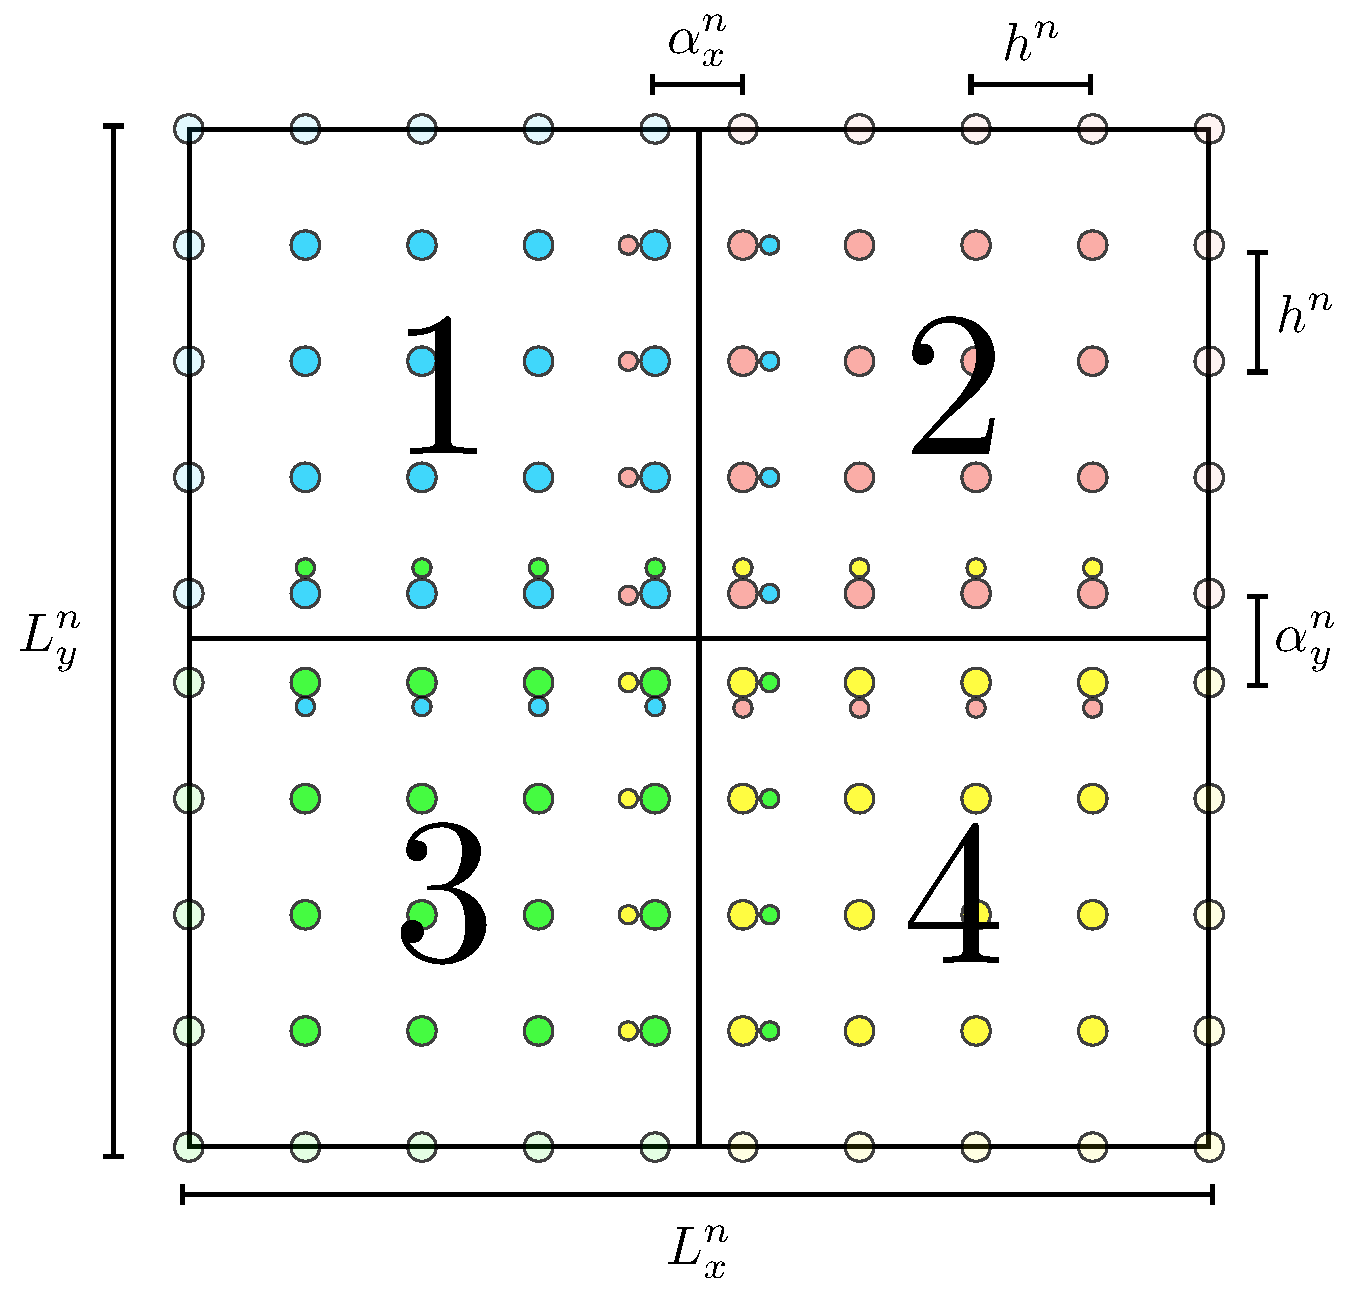
\includegraphics[width=0.5\textwidth]{2DDynamicGrid.pdf}
    \caption{Applying the dynamic grid to a 2D system. Virtual grid points are denoted as smaller circles and boundary points are not included in the calculation (for Dirichlet / simply supported boundary conditions). 
    %Indices along the $x$-direction increment from left to right, and those along the $y$-direction from top to bottom.
    }
    \label{fig:2DGrid}
\end{figure}
%
The systems are subdivided into $M_{x,i}^n$ intervals in the $x$-direction and $M_{y,i}^n$ intervals in the $y$-direction and the spatial indices have the following ranges: $l_i \in\{0, \hdots M_{x,i}^n\}$ and $m_i \in\{0, \hdots M_{y,i}^n\}$. 

Subsystems placed next to each other in the $x$-direction need to have the same number of points in the $y$-direction and vice versa. In other words, the following constraints apply to the number of intervals per subsystem $M_{x, 1}^n = M_{x, 3}^n$, $M_{x, 2}^n = M_{x, 4}^n$, $M_{y, 1}^n = M_{y, 2}^n$, $M_{y, 3}^n = M_{y, 4}^n$. Furthermore, $0<M_{x,1}^n<N_x^n$ and $M_{x,2}^n = N_x^n-M_{x,1}^n$, and $0<M_{y,1}^n<N_y^n$ and $M_{y,3}^n = N_y^n-M_{y,1}^n$.

The grid points of each of the systems are positioned in the $x$-$y$-plane as follows:%, such that the systems in order are top-left, top-right, bottom-left, bottom-right:  
\begin{subequations}
    \begin{align}
        &\!\!\!\left(x_{u_{1, l_1, m_1}}^n, y_{u_{1, l_1, m_1}}^n\right) = \left(l_1h^n, m_1h^n\right),\\
        &\!\!\!\left(x_{u_{2, l_2, m_2}}^n, y_{u_{2, l_2, m_2}}^n\right) =  \left(L_x-(M_{x,2}^n-l_2)h^n, m_2h^n\right),\\
        &\!\!\!\left(x_{u_{3, l_3, m_3}}^n, y_{u_{3, l_3, m_3}}^n\right) = \left(l_3h^n, L_y-(M_{y,3}^n-m_3)h^n\right),\\
        &\!\!\!\begin{aligned}\left(x_{u_{4, l_4, m_4}}^n, y_{u_{4, l_4, m_4}}^n\right) =
        \Big(&L_x-(M_{x,4}^n-l_4)h^n,\\ \qquad &L_y-(M_{y,4}^n-m_4)h^n\Big).\end{aligned}
    \end{align}
\end{subequations}
Notice that, like in the 1D case, the boundary points are fixed at the ends of the domain. If Dirichlet or simply supported boundary conditions are used, one can exclude the boundary points in the calculation and the ranges for the spatial indices become 
\begin{equation}\label{eq:rangesLM}
    \begin{aligned}
        l_1 &= \{1, M_{x,1}^n\}, &\quad m_1 &= \{1, M_{y,1}^n\}, \\
         l_2 &= \{0, M_{x,2}^n-1\}, &\quad m_2 &= \{1, M_{y,2}^n\},\\
        l_3 &= \{1, M_{x,3}^n\},&\quad m_3 &= \{0, M_{y,3}^n-1\},\\
        l_4 &= \{0, M_{x,4}^n-1\}, &\quad m_4 &= \{0, M_{y,4}^n-1\}.
    \end{aligned}
\end{equation}
Finally, one can define the inner boundaries that connect $u_1$ and $u_2$ as the first vertical inner boundary and those connecting $u_3$ and $u_4$ as the second vertical inner boundary. The same can be done for the first and second horizontal inner boundaries, which are those connecting $u_1$ and $u_3$, and $u_2$ and $u_4$, respectively. 

The virtual grid points at the first vertical and horizontal inner boundary are then calculated through
\begin{subequations}\label{eq:connectionInterpol2D}
    \begin{align}
            \!\!\!\!\!\!\!\!&u_{1, M_{x,1}^n+1, m_1}^n = \Aterm_x u_{1, M_{x,1}^n, m_1}^n + u_{2, 0, m_2}^n - \Aterm_x u_{2, 1, m_2}^n,\\
            \!\!\!\!\!\!\!\!&u_{2, -1, m_2}^n = -\Aterm_x u_{1, M_{x, 1}^n-1, m_1}^n + u_{1, M_{x,1}^n, m_1}^n+\Aterm_x u_{2, 0, m_2}^n,\\
            \!\!\!\!\!\!\!\!&u_{1, l_1, M_{y,1}^n+1}^n = \Aterm_y u_{1, l_1, M_{y,1}^n}^n + u_{3, l_3, 0}^n - \Aterm_y u_{3, l_3, 1}^n,\\
           \!\!\!\!\!\!\!\!&u_{3, l_3, -1}^n = -\Aterm_y u_{1, l_1, M_{y, 1}^n-1}^n + u_{1, l_1, M_{y,1}^n}^n+\Aterm_y u_{3, l_2, 0}^n,
    \end{align}
\end{subequations}
respectively, and can be applied in the same manner to the second vertical and horizontal inner boundaries. \SWcomment[$\leftarrow$ possibly elaborate here] Here, 
\begin{equation}\label{eq:axayDef}
    \Aterm_x = \frac{\alpha_x^n-1}{\alpha_x+1}, \qaq \Aterm_y = \frac{\alpha_y^n-1}{\alpha_y^n+1},
\end{equation}
with 
\begin{equation}
    \alpha_x^n = \Nfrac_x^n - N_x^n, \qaq \alpha_y^n = \Nfrac_y^n - N_y^n,
\end{equation}
and fractional number of intervals in the $x$ and $y$-direction $\Nfrac_x^n = L_x^n / h^n$ and $\Nfrac_y^n = L_y^n / h^n$ respectively.

\subsubsection{Matrix Form}
Similar to Eq. \eqref{eq:stackedQ}, one can stack the total state of the system into a single column vector.\footnote{In terms of `column of system no. \#', the order will be: 1, 3, ..., 1, 3, 2, 4, ..., 2, 4.} If Dirichlet or simply supported boundary conditions are used, the total state can then be described as the following $\MtwoD \times 1$ column vector:
\begin{equation}\label{eq:stacked2D}
     \uStack^n = [\v^n, \w^n]^T,
\end{equation}
with $\MtwoD =(M_{x, 1}^n + M_{x, 2}^n) (M_{y, 1}^n + M_{y, 3}^n)$. Here,
\begin{equation}\label{eq:vw}
\begin{aligned}
    \v^n &= [(\v_{1}^n)^T,\hdots, (\v_{M_{x,1}^n}^n)^T]^T, \qaq\\
    \w^n &= [(\w_{0}^n)^T, \hdots, (\w_{M_{x, 2}^n-1}^n)^T]^T,
\end{aligned}
\end{equation}
and
\begin{equation*}
     \v_{j_1^n}^n = [(\u_{1, j_1^n}^n)^T, (\u_{3, j_1^n}^n)^T]^T, \ \ \w_{j_2^n}^n = [(\u_{2, j_2^n}^n)^T, (\u_{4, j_2^n}^n)^T]^T,
\end{equation*}
with $j_1^n = \{1, \hdots, M_{x,1}^n\}$ and $j_2^n = \{0, \hdots, M_{x,2}^n-1\}$. Finally, 
\begin{equation}\label{eq:2DuDefs}
    \begin{aligned}
         \u_{1,l_1}^n &= [u_{1, l_1, 1}^n, \hdots, u_{1, l_1, M_{y, 1}^n}^n]^T,
         \\
         \u_{2,l_2}^n &= [u_{2, l_2, 1}^n, \hdots, u_{2, l_2, M_{y, 2}^n}^n]^T,\\
         \u_{3,l_3}^n &= [u_{3, l_3, 0}^n, \hdots, u_{3, l_3, M_{y, 3}^n-1}^n]^T,\\
         \u_{4,l_4}^n &= [u_{4, l_4, 0}^n, \hdots, u_{1, l_4, M_{y, 4}^n-1}^n]^T.
     \end{aligned}
\end{equation}

\subsubsection{Adding and Removing Points}
Addition and removal of grid points happens in a similar fashion as described in Sec. \ref{sec:addRemove}, the difference being that an entire row or column of grid points affected rather than a single grid point.

Only considering alterations in the left systems, a column can be added to the system by carrying out the following operation on $\v$ in Eq. \eqref{eq:vw}

\begin{equation}
\begin{aligned}
   \v^n &= [(\v^n)^T, \Z^n(I_3^n)^T]^T,\\
   \v^{n-1} &= [(\v^{n-1})^T, \Z^{n-1}(I_3^n)^T]^T
   \end{aligned} \quad \text{if } N_x^n > N_x^{n-1},
\end{equation}
where
\begin{align*}
\Z^n &= [(\v_{M_{x,1}^{n-1}-1}^n)^T, (\v_{M_{x,1}^{n-1}}^n)^T, (\w_{0}^n)^T, (\w_{1}^n)^T], \quad \text{and}\\
\Z^{n-1} &= [(\v_{M_{x,1}^{n-1}-1}^{n-1})^T, (\v_{M_{x,1}^{n-1}}^{n-1})^T, (\w_{0}^{n-1})^T, (\w_{1}^{n-1})^T]
\end{align*}
contain the states of the vertical inner boundaries and their first neighbours in the $x$-direction. 

Only considering alterations in the top systems, a row can be added by carrying out the following operation on $\u_1$ and $\u_2$ in Eq. \eqref{eq:2DuDefs} (done for both $\u^n$ and $\u^{n-1}$) 
\begin{equation*}
    \begin{aligned}
        \u_{1,l_1}^n &= [(\u_{1,l_1}^n)^T, I_3^n \z_{1, l_1}^n]^T,\\
        \u_{2,l_2}^n &= [(\u_{2,l_2}^n)^T, I_3^n \z_{2, l_2}^n]^T,\\
        \u_{1,l_1}^{n-1} &= [(\u_{1,l_1}^{n-1})^T, I_3^n \z_{1, l_1}^{n-1}]^T,\\
        \u_{2,l_2}^{n-1} &= [(\u_{2,l_2}^{n-1})^T, I_3^n \z_{2, l_2}^{n-1}]^T,
    \end{aligned}\quad \text{if } N_y^n > N_y^{n-1},
\end{equation*}
% where the matrix containing the states of the horizontal inner boundaries and their neighbours is defined as
% \begin{equation*}
%     \Z^n = [\z_{1, 1}^n, \hdots, \z_{1, M_{x,1}^{n-1}}^n, \z_{2, 0}^n, \hdots, \z_{M_{x,2}^{n-1}-1}^n],
% \end{equation*}
where 
\begin{align*}
    \z_{1,l_1}^n &= [u_{1, l_1, M_{y,1}^{n-1}-1}^n, u_{1, l_1, M_{y,1}^{n-1}}^n, u_{3, l_1, 0}^n, u_{3, l_1, 1}^n]^T,\\
    \z_{2,l_2}^n &= [u_{2, l_2, M_{y,2}^{n-1}-1}^n, u_{2, l_2, M_{y,2}^{n-1}}^n, u_{4, l_2, 0}^n, u_{4, l_2, 1}^n]^T,\\
    \z_{1,l_1}^{n-1} &= [u_{1, l_1, M_{y,1}^{n-1}-1}^{n-1}, u_{1, l_1, M_{y,1}^{n-1}}^{n-1}, u_{3, l_1, 0}^{n-1}, u_{3, l_1, 1}^{n-1}]^T, \quad \text{and}\\
    \z_{2,l_2}^{n-1} &= [u_{2, l_2, M_{y,2}^{n-1}-1}^{n-1}, u_{2, l_2, M_{y,2}^{n-1}}^{n-1}, u_{4, l_2, 0}^{n-1}, u_{4, l_2, 1}^{n-1}]^T,
\end{align*}
contain the horizontal inner boundaries and their first neighbours in the $y$-direction (the ranges for $l_1$ and $l_2$ are given in Eq. \eqref{eq:rangesLM}).

Removing grid points also happens in a similar fashion to the 1D case. Removing a column from the system happens according to 
\begin{equation}
\begin{aligned}
    \v^n &= [(\v_1^n)^T, \hdots, (\v_{M_{x,1-1}^{n-1}}^n)^T]^T\\
    \v^{n-1} &= [(\v_1^{n-1})^T, \hdots, (\v_{M_{x,1-1}^{n-1}}^{n-1})^T]^T
    \end{aligned}
\quad \text{if } N_x^n < N_x^{n-1}
\end{equation}
and removing a row from the system happens according to

\begin{equation}
    \begin{aligned}
        \u_{1,l_1}^n &= [u_{1,l_1, 1}^n, \hdots, u_{1,l_1, M_{y,1}^{n-1}-1}^n]^T,\\
        \u_{2,l_2}^n &= [u_{2,l_2, 1}^n,\hdots, u^n_{2,l_2, M_{y, 1}^{n-1}-1}]^T,\\
        \u_{1,l_1}^{n-1} &= [u_{1,l_1, 1}^{n-1}, \hdots, u_{1,l_1, M_{y,1}^{n-1}-1}^{n-1}]^T,\\
        \u_{2,l_2}^{n-1} &= [u_{2,l_2, 1}^{n-1},\hdots, u^{n-1}_{2,l_2, M_{y, 1}^{n-1}-1}]^T,
    \end{aligned}\quad \text{if } N_y^n < N_y^{n-1}.
\end{equation}
\subsubsection{State correction}
Like in the 1D case presented in Sec. \ref{sec:stateCorrection}, an artificial spring force can be added to the inner boundaries to prevent audible artifacts when removing grid points. If the state correction is applied to all grid points along the inner boundaries except for those at the intersection of the horizontal and vertical inner boundaries, (i.e., $u_{1, M_{x,1}^n, M_{y,1}^n}^n$, $u_{2, 0, M_{y,2}^n}^n$,$u_{3, M_{x,3}^n, 0}^n$ and $u_{4, 0, 0}^n$) the system can still be solved explicitly. \SWcomment[move to results? $\rightarrow$]It has been found that excluding the state correction at these locations has a minimal effect on the eventual behaviour of the system, and applying the state correction everywhere else already prevents audible artifacts.  

\subsection{2D Wave Equation}
The PDE of the 2D wave equation is defined as
\begin{equation}\label{eq:2DWavePDE}
    \ptt q = c^2 \Delta q,
\end{equation}
with wave speed $c$ (in m/s) and Laplacian
\begin{equation}
    \Delta = \pxx + \pyy.
\end{equation}
Equation \eqref{eq:2DWavePDE} can be discretised to the following FD scheme:
\begin{equation}\label{eq:2DWaveFDS}
    \dtt \qlmn = c^2 \dDelta \qlmn.
\end{equation}
where,
\begin{equation}\label{eq:discLaplacian}
    \dDelta = \dxx + \dyy
\end{equation}
is the discrete Laplacian, and 
\begin{subequations}
\begin{align}
    \pxx q &\approxeq \dxx \qlmn \triangleq \frac{1}{h^2}\left(q_{l+1,m}^n - 2 \qlmn + q_{l-1,m}^n\right),\\
    \pyy q &\approxeq \dxx \qlmn \triangleq \frac{1}{h^2}\left(q_{l,m+1}^n - 2 \qlmn + q_{l,m-1}^n\right).
\end{align}
\end{subequations}
Finally, the stability condition is $h = \sqrt{2}c k$.

\subsubsection{Matrix Form}
Again assuming Dirichlet boundary conditions, one can define matrix forms of $\dxx$ and $\dyy$ similar to Eq. \eqref{eq:dxxMat}, i.e., $(N_x-1)\times(N_x-1)$ matrix $\Dxx$ and $(N_y-1)\times(N_y-1)$ matrix $\Dyy$. These can be used to obtain a matrix form of the discrete Laplacian in Eq. \eqref{eq:discLaplacian} by performing a Kronecker sum \cite{Horn1991} (see Appendix):
\begin{equation}\label{eq:kroneckerSum}
    \DDeltamat = \Dyy \oplus \Dxx,
\end{equation}
and is of size $(N_x+N_y-2)\times (N_x+N_y-2)$.
%
Using same-sized identity matrix $\I = \I_{N_x+N_y-2}$ and the stacked state vector in Eq. \eqref{eq:stackedQ}, the scheme in Eq. \eqref{eq:2DWaveFDS} can then be rewritten in matrix form as
\begin{equation}
    \qq^{n+1} = (2\I + c^2 k^2\DDeltamat)\qq^n - \qq^{n-1}.
\end{equation}
\subsubsection{Applying the Dynamic Grid}
Using the state vector in Eq. \eqref{eq:stacked2D} one can write the update equation of the 2D wave equation including the dynamic grid in matrix form as
\begin{equation}\label{eq:2DwaveDynMatrix}
    \uStack^{n+1} = \left(2\I_\MtwoD + (c^n)^2k^2\DDdelta\right)\uStack^n -\uStack^{n-1}
\end{equation}
with $\MtwoD \times \MtwoD$ matrix
\begin{equation}
    \DDdelta = \DDyy \oplus \DDxx.
\end{equation}
$\DDxx$ and $\DDyy$ include the effect of the interpolation at the inner boundaries presented in Eq. \eqref{eq:connectionInterpol2D} and are as defined in Eq. \eqref{eq:magicMatrix} with $\Aterm_x$ and $\Aterm_y$ as defined in Eq. \eqref{eq:axayDef} respectively. 

\subsection{Thin Plate}
Similar to the stiff string presented in Sec. \ref{sec:stiffString}, one can extend the dynamic grid method to other systems using higher-order spatial derivatives.

Consider the PDE of a thin plate \cite{Morse1968}
\begin{equation}\label{eq:thinPlateFDS}
    \ptt q = -\kappa^2\Delta\Delta q
\end{equation}
where $\kappa$ is (again) a stiffness coefficient (in m$^2$/s). This can be discretised to 
\begin{equation}
    \dtt\qlmn = -\kappa^2\delta_{\Delta\Delta}\qlmn
\end{equation}
where $\delta_{\Delta\Delta} = \delta_{\Delta}\delta_{\Delta},$ and $ h = 2\sqrt{\kappa k}$. 
Eq. \eqref{eq:thinPlateFDS} can we written in matrix form as
\begin{equation}
    \q^{n+1} = \left(2\I - \kappa^2 k^2 \DDeltaDelta\right)\q^n - \q^{n-1}
\end{equation}
where $\I = \I_{N_x + N_y - 2}$ and for simply supported boundary conditions
\begin{equation}
    \DDeltaDelta = \DDeltamat\DDeltamat,
\end{equation}
with $\DDeltamat$ as defined in Eq. \eqref{eq:kroneckerSum}.

The dynamic grid can be applied to this system similar to before as
\begin{equation}\label{eq:thinPlateDynMatrix}
    \uStack^{n+1} = \left(2\I_\MtwoD - (\kappa^n)^2 k^2 \DDDeltaDelta\right)\uStack^n - \uStack^{n-1}
\end{equation}
where for simply supported boundary conditions
\begin{equation}
    \DDDeltaDelta = \DDDelta\DDdelta,
\end{equation}
and is of size $\MtwoD \times \MtwoD$.

\section{ANALYSIS AND RESULTS}\label{sec:analysis}
To evaluate the dynamic grid..

\subsection{Stability Analysis}
Notes:

\SWcomment[I can show numerically that for all dynamic grid update equations (Eqs. \eqref{eq:1DwaveDynMatrix}, \eqref{eq:stiffStringDynMatrix}, \eqref{eq:2DwaveDynMatrix} and \eqref{eq:thinPlateDynMatrix}) written in one-step form, the eigenvalues of matrix $\BB$ (see eq. \eqref{eq:modalAnalysis}) are located on the unit circle for all values of $\alpha^n$ (given that the stability condition is satisfied). However, I can't algebraically prove this. I do know that this shows stability as well as the absence of damping in the system (right?). More importantly, is should I mention this fact somewhere?]

\SWcomment[
Alternatively, I can numerically show that the determinant of $\BB$ is 1, for any value of $\alpha^n$. Hope that that helps to prove something...]

\subsection{Modal Frequencies}

One can retrieve the modal frequencies of the implementation of the dynamic grid by performing a modal analysis of the update equation in matrix form. For reference, these are Eqs. \eqref{eq:1DwaveDynMatrix}, \eqref{eq:stiffStringDynMatrix}, \eqref{eq:2DwaveDynMatrix} and \eqref{eq:thinPlateDynMatrix}. The $p$\th frequency can be calculated as
\begin{equation}\label{eq:modalAnalysis}
    f_p^n = \frac{1}{2 \pi k}\cos^{-1}\left(\frac{1}{2}\text{eig}_p(\BB)\right),
\end{equation}
where $\BB$ is the matrix multiplied onto $\uStack^n$ in each respective update equation and $\text{eig}_p(\cdot)$ denotes the ``$p$\th eigenvalue of".

To determine how accurate the frequency content is, the frequencies obtained in Eq. \eqref{eq:modalAnalysis} can be compared to the modal frequencies that the implementation is expected to have. \SWcomment[not sure if I want to include the following, but just so you know how I did the analysis :) $\rightarrow$]
The expected modal frequencies of a FD scheme as a function of the wave number can be obtained by performing a von Neumann analysis on the discrete scheme. The wave number as a function of physical parameters can then be obtained through a combination of dispersion analysis and modal analysis of the continuous PDE. 

%% other wording
% One can analyse the continuous-time equations and the FD scheme to retrieve the modal frequencies as a function of physical parameters. These will be the expected modal frequencies.

% These can be compared modal frequencies exhibited by the eventual implementation by performing a modal analysis on the update equation in matrix form including the dynamic grid. 

In the following, the difference between the expected modal frequencies and those exhibited by the implementation will be expressed in cents.

In all cases, the following facts apply:
\begin{itemize}
    \item If $\alpha^n$ = 0, the system yields identical behaviour to the original. 
    \item The number of modes is always equal to the number of moving grid points in the system.
    \item The higher the modal number, the higher its frequency deviation.
    \item The higher the number of grid points in the simulation, the less frequency deviation occurs.
    \item The highest deviation amount for one value of $N^n$ happens for $\alpha^n \lesssim 0.25$.
\end{itemize}

% One can retrieve the modal frequencies of a FD scheme by performing a modal analysis on its update equation in matrix form. These can be compared to the expected modal frequencies one can obtain from the continuous 

% \begin{table}[t]
% \tabcolsep8.1pt
% \caption{Tables should have a brief caption. Highlighting the best result(s) is helpful to readers.}
% \label{table:an_example_table}
% {%
% \begin{tabular}{@{}lllc@{}}\toprule
%  & \multicolumn{3}{c}{$\Nfrac$}\\\colrule
%  Model & 15 - 16 & 20 - 21 & 50 - 51  \\\hline
% 1D wave & -67.02 & -54.19 & -25.85 \\
%         Bar & -96.00 & -77.38 & -36.71\botrule
% \end{tabular}}
% \begin{tabnote}
% Note. This table contains several acronyms which should be defined in the paper, when they are first used (but not in the abstract).
% \end{tabnote}
% \end{table}


\begin{table}[h]
    \centering
        \caption{Caption}

    \begin{tabular}{|c|c|c|c|c|}
        \hline & 15 - 16 & 20 - 21 & 50 - 51  \\\hline
        1D wave & -67.02 & -54.19 & -25.85 \\
        Bar & -96.00 & -77.38 & -36.71\\\hline
    \end{tabular}
    \label{tab:my_label}
\end{table}

\subsubsection{1D Wave Equation}

1D wave $\Nfrac^n = 15 \rightarrow \Nfrac^n = 16$ 

\subsubsection{Stiff String}

Cent deviation:

\subsection{State Correction}
In the 1D case, the state correction presented in Sec. \ref{sec:stateCorrection} does not affect the modal content 
\section{DISCUSSION}\label{sec:discussion}
Damping can easily be added to the systems presented in Sections \ref{sec:dynamicGrid} and \ref{sec:2D}.

Frequency deviations occur in higher frequency ranges and are thus much less perceptually relevant than 

Notes:

Multiplying the average slope of the line that connects the (higher-frequency) minima of each deviation in Hz by the values of $\Nfrac$ that causes these minima, yields lines that are bounded by the samplerate...



\section{CONCLUSION}\label{sec:conclusion}
Not limited to two dimensions, could extend to 3D systems

Real-time implementation and control, such that a player can `mould' their instrument while performing, potentially discovering new ways of expression with the instrument at hand.   

\section{ACKNOWLEDGMENTS}
This  work  has  been  funded  in  part  by  the European Art-Science-Technology Network for Digital Creativity (EASTN-DC). Thanks to the DAFx20in21 committee for \SWcomment[supporting this publication to be open access].

% \bibliography{jaes.bib}
% \bibliographystyle{jaes.bst}

\appendix
\section*{APPENDIX: KRONECKER SUM}\label{app:kronecker}
To obtain the matrix form of the discrete Laplacian in Eq. \eqref{eq:kroneckerSum} the Kronecker product and Kronecker sum need to be introduced. The Kronecker product between two matrices is \cite{Horn1991}
\begin{equation}
    \A_{M\times N} \otimes \B_{K\times L} = \begin{bmatrix}
        a_{11}\B & \hdots & a_{1N}\B\\
        \vdots & \ddots & \vdots\\
        a_{M1}\B & \hdots & a_{MN}\B\\
    \end{bmatrix}_{MK \times NL},
\end{equation}
and the kronecker sum between two square matrices is \cite{Hamilton2016}
\begin{equation}\label{eq:kronSum}
    \A_{M \times M} \oplus \B_{N \times N} = \I_N\otimes \A + \B \otimes\I_M.
\end{equation}

%Biography
 \biography{Silvin Willemsen}{JAESheadshotSilvin.jpg}{Silvin Willemsen is a Postdoctoral Researcher at Aalborg University in Copenhagen, Denmark. He received his MSc. in Sound and Music Computing from Aalborg University in 2017. In 2018, he was appointed as a PhD Stipend at the Department of Architecture, Design and Media Technology at Aalborg University Copenhagen and was affiliated with the Multisensory Experience Lab. In 2021 he received his PhD degree and continues to work in the field of physical modelling for musical instrument simulations.}
 \biography{Stefan Bilbao}{}{Lorem ipsum dolor sit amet, consectetur adipiscing elit. Integer pharetra massa nec erat elementum, non lacinia massa vehicula. Aenean lobortis pretium ex quis rutrum. Donec ut vehicula sem. Vestibulum sem sem, imperdiet in enim id, convallis porttitor velit. Curabitur elementum tincidunt diam. Donec pulvinar rutrum nisi, eu fringilla mauris gravida dignissim. Ut in nibh vehicula, congue lectus et, feugiat libero. Phasellus tempus turpis at lobortis condimentum. Proin egestas luctus aliquam. Cras consequat, lorem sed facilisis accumsan, felis lacus facilisis lectus, at fringilla velit turpis et dui.}
 \biography{Michele Ducceschi}{}{Lorem ipsum dolor sit amet, consectetur adipiscing elit. Integer pharetra massa nec erat elementum, non lacinia massa vehicula. Aenean lobortis pretium ex quis rutrum. Donec ut vehicula sem. Vestibulum sem sem, imperdiet in enim id, convallis porttitor velit. Curabitur elementum tincidunt diam. Donec pulvinar rutrum nisi, eu fringilla mauris gravida dignissim. Ut in nibh vehicula, congue lectus et, feugiat libero. Phasellus tempus turpis at lobortis condimentum. Proin egestas luctus aliquam. Cras consequat, lorem sed facilisis accumsan, felis lacus facilisis lectus, at fringilla velit turpis et dui.}
 \biography{Stefania Serafin}{}{Lorem ipsum dolor sit amet, consectetur adipiscing elit. Integer pharetra massa nec erat elementum, non lacinia massa vehicula. Aenean lobortis pretium ex quis rutrum. Donec ut vehicula sem. Vestibulum sem sem, imperdiet in enim id, convallis porttitor velit. Curabitur elementum tincidunt diam. Donec pulvinar rutrum nisi, eu fringilla mauris gravida dignissim. Ut in nibh vehicula, congue lectus et, feugiat libero. Phasellus tempus turpis at lobortis condimentum. Proin egestas luctus aliquam. Cras consequat, lorem sed facilisis accumsan, felis lacus facilisis lectus, at fringilla velit turpis et dui.}
\end{document}
